\documentclass{article}
\usepackage{nips11submit_e,times}
\nipsfinaltrue
%\usepackage{amsmath,amssymb,amsthm,enumerate,natbib,color,bbm,ifthen,graphicx,overpic}
% JB: I don't have bbm and paper doesn't seem to need it. can we leave it out of the list?
\usepackage{amsmath,amssymb,amsthm,enumerate,natbib,color,ifthen,graphicx,overpic}

% VERSION FOR WEB READING SHOULD USE HYPERREF
%\usepackage[colorlinks=false]{hyperref}

% VERSION FOR PRINTING SHOULD USE URL (looks nicer)
\usepackage{url}

\setlength{\parskip}{\medskipamount}
\setlength{\parindent}{0pt}
\usepackage{myAlgorithm}
\usepackage{notations}
\usepackage{capt-of}
\usepackage{natbib}

\title{Algorithms for Hyper-Parameter Optimization}
\author{
James Bergstra\\ %\thanks{\url{http://people.fas.harvard.edu/$\sim$bergstra}} \\
The Rowland Institute\\
Harvard University\\
%Cambridge, MA 02142 \\
\texttt{bergstra@rowland.harvard.edu} \\
\And
R{\'e}mi Bardenet \\
Laboratoire de Recherche en Informatique\\
Universit{\'e} Paris-Sud \\
\texttt{bardenet@lri.fr} \\
\AND
Yoshua Bengio \\
D{\'e}pt. d'Informatique et Recherche Op{\'e}rationelle \\
Universit{\'e} de Montr{\'e}al\\
\texttt{yoshua.bengio@umontreal.ca} \\
\And
Bal{\'a}zs K{\'e}gl \\
Linear Accelerator Laboratory \\
Universit{\'e} Paris-Sud, CNRS \\
\texttt{balazs.kegl@gmail.com}
}
\newcommand{\fix}{}%{\marginpar{FIX}}
\newcommand{\fixme}[1]{}%{{\bf FIXME: {#1}}} %unlike \fix, this works in captions
\newcommand{\new}{\marginpar{NEW}}

\newcommand{\algorandom}{random}

\newcommand{\vs}[1]{\vspace*{-#1mm}}
\newcommand{\Bs}{\vs{2}}
\newcommand{\as}{\vs{1}}
\newcommand{\Bss}{\vs{1}}
\newcommand{\ass}{\vs{0.7}}
\renewcommand{\citet}{\cite}

\begin{document}
\maketitle
\begin{abstract}
\vs{2}
    Several recent advances to the state of the art in image classification benchmarks have come
    from better configurations of existing techniques rather than novel approaches to
    feature learning.
    %Only by making hyper-parameter optimization a formal component of
    %learning algorithms can we systematically investigate how CPU resources should be
    %allocated between hyper-parameter exploration and hyper-parameter evaluation.
    Traditionally,
    hyper-parameter optimization has been the job of humans because they can be very efficient in regimes where only a few trials are possible.
    Presently, computer clusters and GPU processors make it possible to run more trials
    and we show that algorithmic approaches can find better results.
    We present hyper-parameter optimization results on tasks of training neural networks and deep belief networks (DBNs).
    We optimize hyper-parameters using random search
    and two new greedy sequential methods based on the expected improvement criterion.
    Random search has been shown to be sufficiently efficient for learning neural networks for several datasets,
    but we show it is unreliable for training DBNs.
    The sequential algorithms are applied to the most difficult DBN learning problems from
    \cite{Larochelle+etal:2007} and find significantly better results than the best previously reported.
    This work contributes novel techniques for making response surface models
    $P(y|x)$ in which many elements of hyper-parameter assignment ($x$) are known to be irrelevant
    given particular values of other elements.
\vs{3}
\end{abstract}

\Bs
\section{Introduction}
\as

Models such as Deep Belief Networks (DBNs)~\citep{hinton+osindero+teh:2006},
stacked denoising autoencoders~\citep{vincent+larochelle+lajoie+bengio+manzagol:2010},
convolutional networks~\citep{lecun+bottou+bengio+haffner:1998},
as well as classifiers based on sophisticated feature extraction techniques % such as mcRBMs~\citep{ranzato+hinton:2010}
have from ten to perhaps fifty hyper-parameters, depending on how
the experimenter chooses to parametrize the model, and how many
hyper-parameters the experimenter chooses to fix at a reasonable default.
The difficulty of tuning these models makes published results difficult to
reproduce and extend, and makes even the original investigation of such methods more
of an art than a science.

Recent results such as
\citet{Pinto-2009}, \citet{coates+lee+ng:2010}, and \citet{coates+ng:2011}
demonstrate that the challenge of hyper-parameter optimization
in large and multilayer models is a direct impediment to scientific progress.
These works
have advanced state of the art performance on image classification problems
by more concerted hyper-parameter optimization in simple algorithms,
rather than by innovative modeling or machine learning strategies.
It would be wrong to conclude from a result such as \citet{Pinto-2009}
that feature learning is useless.
Instead, hyper-parameter optimization should be regarded as
a formal outer loop in the learning process.
A learning algorithm,
as {\em a functional from data to classifier} (taking classification problems as an example),
includes a budgeting choice of how many CPU cycles are to be spent on hyper-parameter exploration,
and how many CPU cycles are to be spent evaluating each hyper-parameter choice (i.e. by
tuning the regular parameters).
The results of \citet{Pinto-2009} and \citet{coates+ng:2011} suggest that
with current generation hardware such as large computer clusters and GPUs,
the optimal allocation of CPU cycles includes more hyper-parameter exploration
than has been typical in the machine learning literature.

Hyper-parameter optimization is the problem of optimizing a loss function
over a graph-structured configuration space.
In this work we restrict ourselves to tree-structured configuration spaces.
Configuration spaces are
tree-structured in the sense that some leaf variables (e.g. the number of
hidden units in the 2nd layer of a DBN) are only well-defined when node
variables (e.g. a discrete choice of how many layers to use) take
particular values. Not only must a hyper-parameter optimization algorithm
optimize over variables which are discrete, ordinal, and continuous, but
it must simultaneously choose which variables to optimize.

In this work we define a configuration space by a generative process for
drawing valid samples.  Random search is the algorithm of drawing
hyper-parameter assignments from that process and evaluating them.  Optimization algorithms
work by identifying hyper-parameter assignments that
could have been drawn, and that appear promising on the basis of the loss
function's value at other points.  This paper makes two contributions:
1) Random search is competitive with the manual optimization of DBNs in
\citet{Larochelle+etal:2007}, and 2) Automatic sequential optimization
outperforms both manual and random search.
% REPLACED ENUMERATION BY INLINE LIST
%\begin{enumerate}
%\item Random search is competitive with the manual optimization of DBNs in
%\citet{Larochelle+etal:2007}.
%\item Automatic sequential optimization outperforms both manual and random search.
%\end{enumerate}

Section \ref{sec:smbo} covers sequential model-based
optimization, and the expected improvement criterion.
Section \ref{ss:GPs} introduces a Gaussian Process based hyper-parameter
optimization algorithm.
Section \ref{sec:TPE} introduces a second approach based on adaptive Parzen windows.
Section \ref{sec:random}  describes the problem of DBN hyper-parameter
optimization, and shows the efficiency of random search.
Section \ref{sec:exp} shows the efficiency of sequential optimization on the
two hardest datasets according to random search.
The paper concludes with discussion of results and concluding remarks in
Section~\ref{sec:discussion} and Section~\ref{sec:conclusion}.

\Bs
\section{Sequential Model-based Global Optimization}
\as
\label{sec:smbo}

Sequential Model-Based Global Optimization (SMBO) algorithms have been used in many applications
where evaluation of the fitness function is expensive~\citep{hutter:2009,hutter+hoos+leyton+brown:2011}.
In an application where the true fitness function
$f:\cX\rightarrow \mathbb{R}$ is costly to evaluate,
model-based algorithms approximate $f$
with a surrogate that is cheaper to evaluate.
Typically the inner loop in an SMBO algorithm is the numerical optimization of this surrogate,
or some transformation of the surrogate.
The point $x^*$ that maximizes the surrogate (or its transformation) becomes the proposal
for where the true function $f$ should be evaluated.
This active-learning-like algorithm template is summarized in Figure~\ref{f:genericAlgo}.
SMBO algorithms differ in
what criterion they optimize to obtain $x^*$ given a model (or surrogate) of $f$,
and in they model $f$ via observation history ${\cal H}$.

%\setlength{\algowidth}{0.95\textwidth}
\begin{figure}[!ht]
\vs{2}
\centerline{
\begin{algorithm}{$\Algo{SMBO}\big(f,M_0, T,S \big)$}
\Aitem $\cH \setto \emptyset$,
\Aitem For $t \setto 1$~\To~$T$,
\Aitem \label{ai:candidate}\mt $x^*~\setto~\operatorname{argmin}_{x}~S(x, M_{t-1})$,
\Aitem \mt Evaluate $f(x^*)$, \mt \algoremark{Expensive step}
\Aitem \mt $\cH \setto \cH \cup (x^*,f(x^*))$,
\Aitem \mt \label{ai:update} Fit a new model $M_t$ to $\cH$.
\Aitem \Return $\cH$
\end{algorithm}
}
\vs{2}
\caption{The pseudo-code of generic Sequential Model-Based
  Optimization.}
\label{f:genericAlgo}
\vs{0}
\end{figure}

The algorithms in this work optimize the criterion of Expected Improvement
(EI)~\cite{Jon01}.
Other criteria have been suggested, such as
Probability of Improvement and Expected Improvement~\citep{Jon01},
minimizing the Conditional Entropy of the Minimizer~\citep{ViVaWa06},
and the bandit-based criterion described in \cite{SrKrKaSe10}.
We chose to use the EI criterion in our work because it is intuitive, and has
been shown to work well in a variety of settings.
We leave the systematic exploration of improvement criteria for future work.
Expected improvement is the expectation under some model $M$ of
$f: {\cal X} \rightarrow \mathbb{R}^N$ that $f(x)$ will exceed (negatively) some threshold
$y^*$:
\begin{equation}
\vs{.5}
\text{EI}_{y^*}(x):=\int_{-\infty}^{\infty} \max(y^* - y, 0) p_M(y\vert x) dy.
\label{e:EI}
\vs{.5}
\end{equation}

The contribution of this work is two novel strategies for
approximating $f$ by modeling $\cal H$:
a hierarchical Gaussian Process and a tree-structured Parzen estimator.
These are described in Section~\ref{ss:GPs} and Section~\ref{sec:TPE}
respectively.

\Bs
\section{The Gaussian Process Approach (GP)}
\as
\label{ss:GPs}
Gaussian Processes have long been recognized as a good method for modeling
loss functions in model-based optimization literature \cite{MoTiZi78}.
Gaussian Processes (GPs, \cite{RaWi06}) are priors over functions that are
{\it closed under sampling}, which means that if the prior
distribution of $f$ is believed to be a GP with mean $0$ and kernel
$k$, the conditional distribution of $f$ knowing a sample
$\cH = (x_i,f(x_i))_{i=1}^n$ of its
values is also a GP, whose mean and covariance function are
analytically derivable. GPs with generic mean functions can in
principle be used, but it is simpler
and sufficient for our purposes to only consider zero mean processes.
We do this by centering the function values in the considered data
sets. Modelling e.g. linear trends in the GP mean leads to
undesirable extrapolation in unexplored regions during SMBO~\cite{GiDuBaCaRo09}.

The above mentioned closedness property, along
with the fact that GPs provide an assessment of prediction uncertainty incorporating the
effect of data scarcity, make the GP an elegant candidate for both
finding candidate $x^*$ (Figure~\ref{f:genericAlgo}, step 3) and
fitting a model $M_t$ (Figure~\ref{f:genericAlgo}, step~\ref{ai:update}).
The runtime of each iteration of
the GP approach scales cubically in $|\cH|$ and linearly in
the number of variables being optimized, however the expense of the function
evaluations $f(x^*)$ typically dominate even this cubic cost.

\Bss
\subsection{Optimizing EI in the GP}
\ass
\label{ss:ea}

We model $f$ with a GP and set $y^*$ to the best value found
after observing $\cH$: $y^*=\min\{
f(x_i),1\leq i\leq n\}$. The model $p_M$ in \eqref{e:EI} is then the
posterior GP knowing $\cH$. The EI function in $\eqref{e:EI}$
encapsulates a compromise between
regions where the mean function is
close to or better than $y^*$ and
under-explored regions where the uncertainty is high.

EI functions are usually optimized with an exhaustive grid search
over the input space, or a Latin Hypercube search in
higher dimensions. However, some information on the landscape of the
EI criterion can be derived from simple computations \cite{BaKe10}: 1) it is
always non-negative and zero at training points from $\mathcal{D}$, 2) it
inherits the smoothness of the kernel $k$, which is
in practice often at least once differentiable, and noticeably, 3) the
EI criterion is likely to be highly multi-modal, especially as the number of
training points increases. The authors of \cite{BaKe10} used the
preceding remarks on the landscape of EI to design an evolutionary
algorithm with mixture search, specifically aimed at optimizing EI,
that is shown to outperform exhaustive search for a given budget in EI
evaluations. We borrow here their approach and go one step further. We keep the
Estimation of Distribution (EDA, \cite{LaLo01}) approach on the discrete
part of our input space (categorical and
discrete hyper-parameters), where we sample candidate points according
to binomial distributions, while we use the Covariance Matrix Adaptation -
Evolution Strategy (CMA-ES, \cite{Han06}) for the remaining part of
our input space (continuous hyper-parameters). CMA-ES is a
state-of-the-art gradient-free evolutionary algorithm for optimization on continuous
domains, which has been shown to outperform the Gaussian search
EDA. Notice that such a gradient-free approach allows
non-differentiable kernels for the GP regression. We do not take on the use
of mixtures in \cite{BaKe10}, but rather restart the local searches
several times, starting from promising places. The use of tesselations
suggested by \cite{BaKe10} is prohibitive here, as our task often means
working in more than 10 dimensions, thus we start each local search at
the center of mass of a simplex with vertices randomly picked among the training points.

Finally, we remark that all hyper-parameters are not relevant for each
point. For example, a DBN with only
one hidden layer does not have parameters associated to a second or
third layer. Thus it is not enough to place one GP over the entire
space of hyper-parameters. We chose to group the hyper-parameters by
common use in a tree-like fashion and place different independent GPs
over each group. As an example, for DBNs, this means placing one GP over common
hyper-parameters, including categorical parameters that indicate what
are the {\it conditional} groups to consider, three GPs on the
parameters corresponding to each of the three layers, and a few 1-dimensional GPs
over individual conditional hyper-parameters, like ZCA
energy (see Table~\ref{tbl:dbnprior} for DBN parameters).

\Bss
\section{Tree-structured Parzen Estimator Approach (TPE)}
\label{sec:TPE}
\ass

Anticipating that our hyper-parameter optimization tasks will mean high
dimensions and small fitness evaluation budgets, we now turn to
another modeling strategy and EI optimization scheme for the SMBO algorithm.
Whereas the Gaussian-process based approach modeled $p(y|x)$ directly,
this strategy models $p(x|y)$ and $p(y)$.

Recall from the introduction that the configuration space $\cX$ is described
by a graph-structured generative process
(e.g. first choose a number of DBN layers, then choose the parameters for each).
The tree-structured Parzen estimator (TPE) models $p(x|y)$ by
transforming that generative process, replacing the distributions of the configuration prior
with non-parametric densities.
In the experimental section, we will see that the configuation space is described using
uniform, log-uniform, quantized log-uniform, and categorical variables.
In these cases, the TPE algorithm makes the following replacements:
uniform $\rightarrow$ truncated Gaussian mixture,
log-uniform $\rightarrow$ exponentiated truncated Gaussian mixture,
categorical $\rightarrow$ re-weighted categorical.
Using different observations $\{x^{(1)},...,x^{(k)}\}$ in the non-parametric densities, these substitutions represent a {\em learning algorithm}
that can produce a variety of densities over the configuration space $\cX$. 
The TPE defines $p(x|y)$ using two such densities:
\begin{equation}
p(x|y) = \begin{cases}
   \ell(x) & \text{if $y < y^*$} \\
   g(x) & \text{if $y \geq y^*$},
   \end{cases}
\end{equation}
where $\ell(x)$ is the density formed by using the observations $\{x^{(i)}\}$ such that corresponding loss $f(x^{(i)})$ was less than $y^*$
and $g(x)$ is the density formed by using the remaining observations.
Whereas the GP-based approach favoured quite an aggressive $y^*$ (typically less than the best observed loss), the TPE
algorithm depends on a $y^*$ that is larger than the best observed $f(x)$ so that some points can be used to form $\ell(x)$.
The TPE algorithm chooses $y^*$ to be some quantile $\gamma$ of the observed $y$ values,
so that $p(y < y^*) = \gamma$, but no specific model for $p(y)$ is necessary.
By maintaining sorted lists of observed variables in $\cH$, the runtime of
each iteration of the TPE algorithm can scale linearly in $|\cH|$ and linearly in
the number of variables (dimensions) being optimized.

%Now, given a threshold $y^*$ under which you consider there's an improvement, there are two regions of interest:
%$G_{y^*} := \{(x,f(x))\in\cX\times\mathbb{R}: f(x) \geq y^*\}\text{ and  }L_{y^*} = \{(x,f(x))\in\cX\times\mathbb{R}: y<y^*\}$.

\subsection{Optimizing EI in the TPE algorithm}

The parametrization of $p(x, y)$ as $p(y)p(x|y)$ in the TPE algorithm was
chosen to facilitate the optimization of EI.
\begin{align}
    \mathrm{EI}_{y^*}(x)
    = \int_{-\infty}^{y^*} (y^* - y)p(y|x) dy
    = \int_{-\infty}^{y^*} (y^* - y) \frac{p(x|y)p(y)}{p(x)}
    dy
\end{align}
By construction, $\gamma = p(y<y^*)$ and
$
%\vs{.5}
p(x) = \int_\mathbb{R} p(x\vert y) p(y) dy = \gamma \ell(x) +
(1-\gamma) g(x).
%\vs{.5}
$
Therefore
\begin{eqnarray}
%\vs{.5}
\int_{-\infty}^{y^*} (y^* - y) p(x|y)p(y) dy &=&
\ell(x)\int_{-\infty}^{y^*} (y^* - y) p(y) dy\nonumber= \gamma y^*\ell(x) - \ell(x)\int_{-\infty}^{y^*} p(y)dy,
%\vs{.5}
\end{eqnarray}
so that finally
%\begin{eqnarray*}
%\vs{.5}
$
EI_{y^*}(x) = \frac{\gamma y^*\ell(x) - \ell(x)\int_{-\infty}^{y^*} p(y)dy}{\gamma \ell(x) +
(1-\gamma) g(x)}
\propto \left( \gamma + \frac{g(x)}{\ell(x)}(1-\gamma)\right)^{-1}.
$
%\vs{.5}
%\end{eqnarray*}
This last expression shows that to maximize improvement we would like
points $x$ with high probability under $\ell(x)$ and low probability
under $g(x)$.
The tree-structured form of $\ell$ and $g$ makes it easy to draw many candidates according to $\ell$ and evaluate them according to $g(x)/\ell(x)$.
On each iteration, the algorithm returns the candidate $x^*$ with the greatest EI.
%together these steps reveal a candidate with high EI. Note finally
%that the choice of the quantile $\gamma\in[0,1]$ is left free to the user.

\Bss
\subsection{Details of the Parzen Estimator}
\ass

The models $\ell(x)$ and $g(x)$ are hierarchical processes involving discrete-valued and continuous-valued variables.
The Adaptive Parzen Estimator yields a model over $\cX$ by placing density in
the vicinity of $K$ observations ${\cal B} = \{x^{(1)}, ..., x^{(K)}\} \subset
\cH$.
Each continuous hyper-parameter was specified by a uniform prior over some
interval $(a, b)$,
or a Gaussian, or a log-uniform distribution.
The TPE substitutes an equally-weighted mixture of that prior with
Gaussians
centered at each of the $x^{(i)} \in {\cal B}$.
The standard deviation of each Gaussian was set to the greater of the
distances to the left and right neighbor, but clipped to remain in a
reasonable range.
In the case of the uniform, the points $a$ and $b$ were considered to be potential neighbors.
For discrete variables, supposing the prior was a vector of $N$ probabilities $p_i$,
the posterior vector elements were proportional to $Np_i + C_i$ where $C_i$
counts the occurrences of choice $i$ in $\cal B$.
The log-uniform hyper-parameters were treated as uniforms in the log domain.

\Bs
\section{Random Search for Hyper-Parameter Optimization in DBNs}
\as
\label{sec:random}

%After the initial random sampling, the TPE algorithm switches to the use of EI based on $\ell(x)$ and $g(x)$.
%Until there are at least a few
%For the first few trials (a hyper-parameter of the TPE),
%the TPE algorithm drew from the initial distribution defined in Table~\ref{tbl:dbnprior}.

One simple, but recent step toward formalizing hyper-parameter optimization is
the use of random search~\citet{Pinto-2009}.
\citet{Bergstra+Bengio:2011snowbird} showed that random search was much more
efficient than grid search for optimizing the parameters of one-layer neural
network classifiers.
In this section, we evaluate random search for DBN
optimization, compared with the sequential grid-assisted manual search
carried out in \citet{Larochelle+etal:2007}.


\begin{table}
\vs{4}
    \caption{Distribution over DBN hyper-parameters for random sampling.
    Options separated by ``or''  such as pre-processing (and including the random seed) are weighted equally.
    Symbol $U$ means uniform, $\mathcal{N}$ means Gaussian-distributed, and $\log U$ means uniformly distributed in the log-domain.
    CD (also known as CD-1) stands for contrastive divergence, the algorithm used to initialize the layer parameters of the DBN.
    %and the distribution used by the \algorandom\ algorithm.
    }
    \label{tbl:dbnprior}
    \centering
    \begin{tabular}{llp{.1in}ll}
        \multicolumn{2}{c}{{\bf Whole model}} & & \multicolumn{2}{c}{\bf Per-layer} \\
        Parameter & Prior & & Parameter & Prior \\
        \hline
        pre-processing & raw or ZCA & & n. hidden units & $\log U(128, 4096)$\\
        ZCA energy & $U(.5, 1)$ & & $W$ init & $U(-a,a)$ or $\mathcal{N}(0, a^2)$ \\
        random seed & 5 choices & & $a$ & algo A or B (see text)\\
        classifier learn rate & $\log U(0.001, 10)$ & & algo A coef& $U(.2,2)$\\
        classifier anneal start & $\log U(100, 10^4)$ & & CD epochs & $\log U(1, 10^4)$\\
        classifier $\ell_2$-penalty & 0 or $\log U(10^{-7}, 10^{-4})$ & & CD learn rate & $\log U(10^{-4},1)$ \\
        n. layers & 1 to 3 & & CD anneal start & $\log U(10, 10^4)$ \\
        batch size & 20 or 100 & & CD sample data & yes or no \\
        \hline
    \end{tabular}
\vs{4}
\end{table}


We chose the prior listed in Table~\ref{tbl:dbnprior} to define the search
space over DBN configurations.
The details of the datasets, the DBN model, and the greedy layer-wise training procedure based on CD
are provided in \cite{Larochelle+etal:2007}.
This prior corresponds to the search space of \cite{Larochelle+etal:2007}
except for the following differences:
(a) we allowed for ZCA pre-processing~\citep{hyvarinen+oja:2000},
(b) we allowed for each layer to have a different size,
(c) we allowed for each layer to have its own training parameters for CD,
(d) we allowed for the possibility of treating the continuous-valued data
as either as Bernoulli means (more theoretically correct)
or Bernoulli samples (more typical) in the CD algorithm, and
(e) we did not discretize the possible values of real-valued hyper-parameters.
These changes expand the hyper-parameter search problem,
while maintaining the original hyper-parameter search space as a subset of the expanded search space.

The results of this preliminary random search are in Figure~\ref{fig:dbn_random_efficiency}.
Perhaps surprisingly, the result of manual search can be reliably matched with 32 random trials for several datasets.
The efficiency of random search in this setting is explored further in
\citet{bergstra+bengio:2012accepted}.
Where random search results match human performance,
it is not clear from Figure~\ref{fig:dbn_random_efficiency}
whether the reason is that it searched the original space as efficiently,
or that it searched a larger space where good performance is easier to find.
But the objection that random search is somehow cheating by searching a larger space is backward --
the search space outlined in Table~\ref{tbl:dbnprior} is a natural description
of the hyper-parameter optimization problem, and the restrictions to that
space by~\citet{Larochelle+etal:2007} were presumably made to simplify
the search problem and make it tractable for grid-search assisted manual search.
Critically, both methods train DBNs on the same datasets.

The results in Figure~\ref{fig:dbn_random_efficiency} indicate that
hyper-parameter optimization is harder for some datasets.
For example, in the case of the ``MNIST rotated background images'' dataset ({\bf MRBI}),
random sampling appears to converge to a maximum relatively quickly (best
models among experiments of 32 trials show little variance in performance),
but this plateau is lower than what was found by manual search.
In another dataset ({\bf convex}), the random sampling procedure exceeds the performance of manual search, but is slow to converge to any sort of plateau.
There is considerable variance in generalization when the best of 32 models is selected.
This slow convergence indicates that better performance is probably available, but we need to search the configuration space more efficiently to find it.
The remainder of this paper explores sequential optimization strategies for hyper-parameter optimization for these two datasets: {\bf convex} and {\bf MRBI}.

\begin{figure}
\vs{2}
\centering
\begin{minipage}{0.9\linewidth}
    \centering
    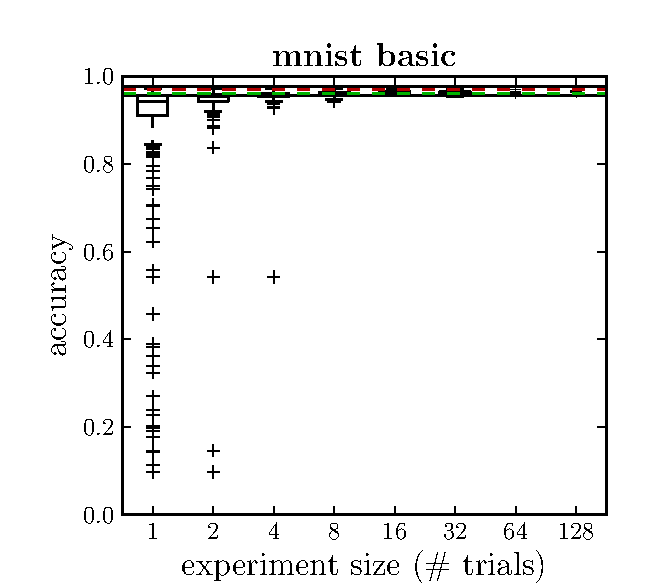
\includegraphics[scale=0.37]{figures/dbn_efficiency/dbn_efficiency_mnist_basic}
    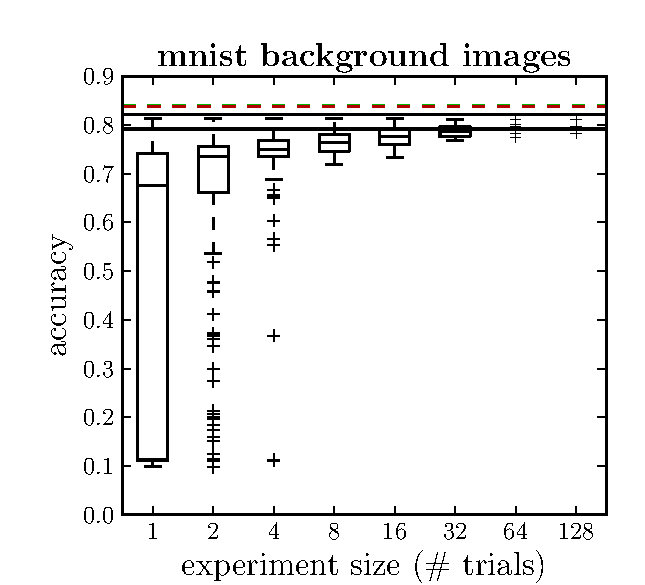
\includegraphics[scale=0.37]{figures/dbn_efficiency/dbn_efficiency_mnist_background_images}
    %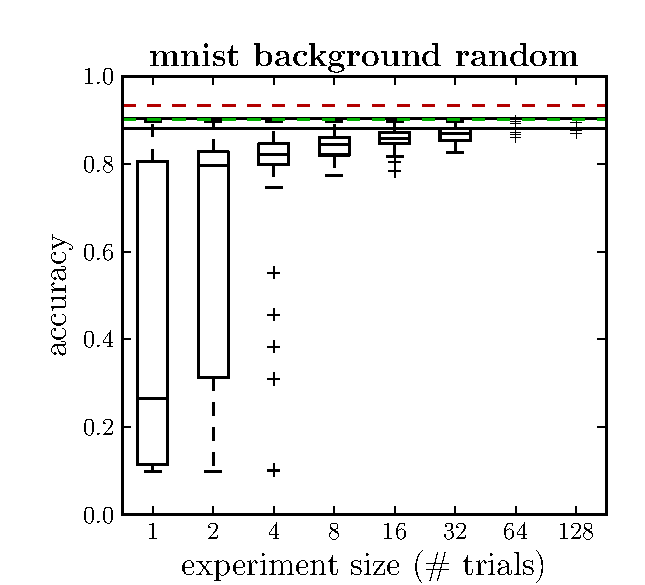
\includegraphics[scale=0.33]{figures/dbn_efficiency/dbn_efficiency_mnist_background_random}
    %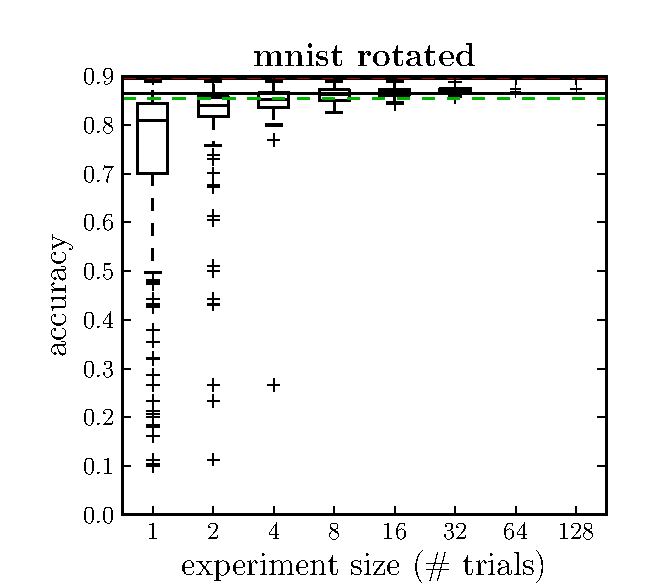
\includegraphics[scale=0.33]{figures/dbn_efficiency/dbn_efficiency_mnist_rotated}
    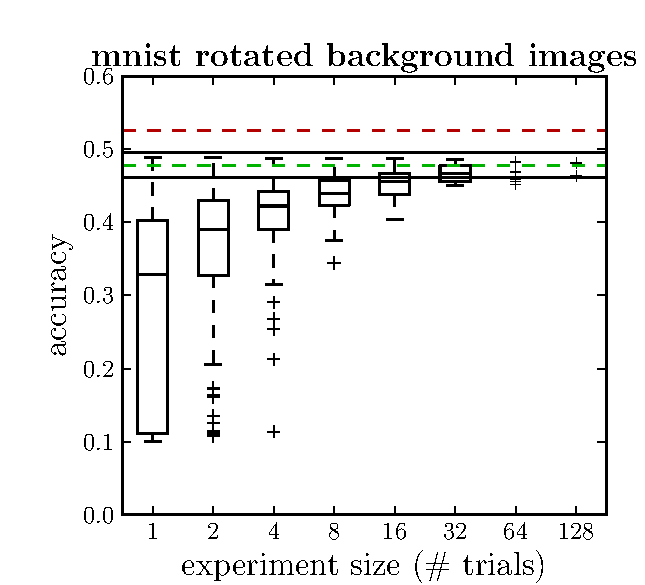
\includegraphics[scale=0.37]{figures/dbn_efficiency/dbn_efficiency_mnist_rotated_background_images}
    %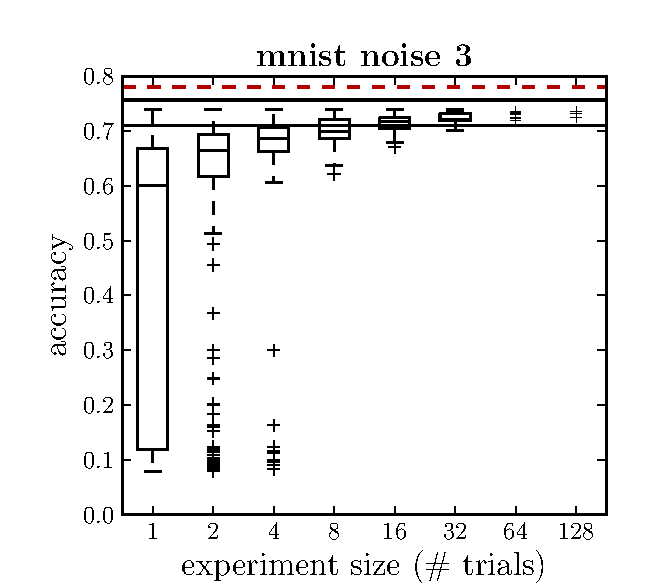
\includegraphics[scale=0.3]{figures/dbn_efficiency/dbn_efficiency_mnist_noise_3}
    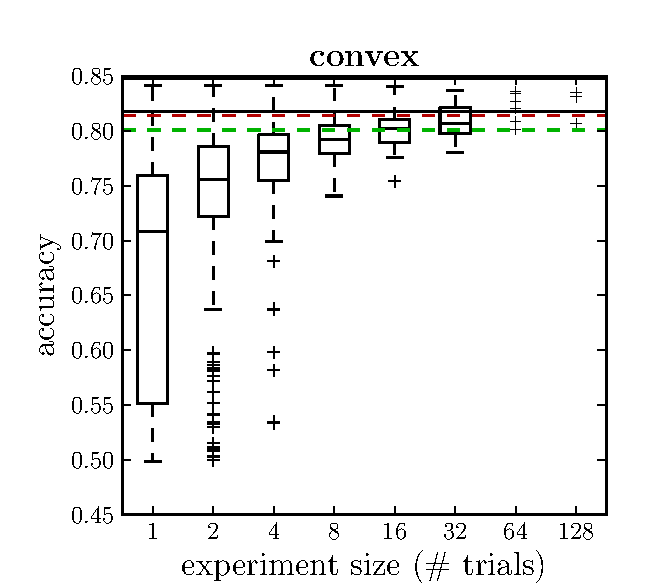
\includegraphics[scale=0.37]{figures/dbn_efficiency/dbn_efficiency_convex}
    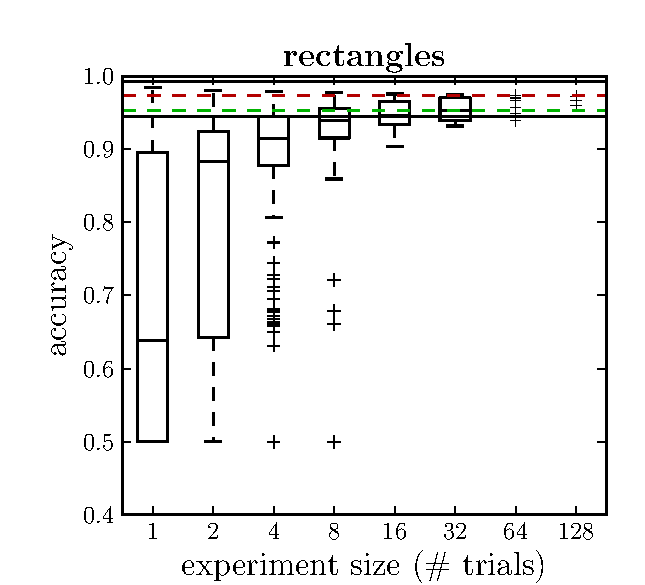
\includegraphics[scale=0.37]{figures/dbn_efficiency/dbn_efficiency_rectangles}
    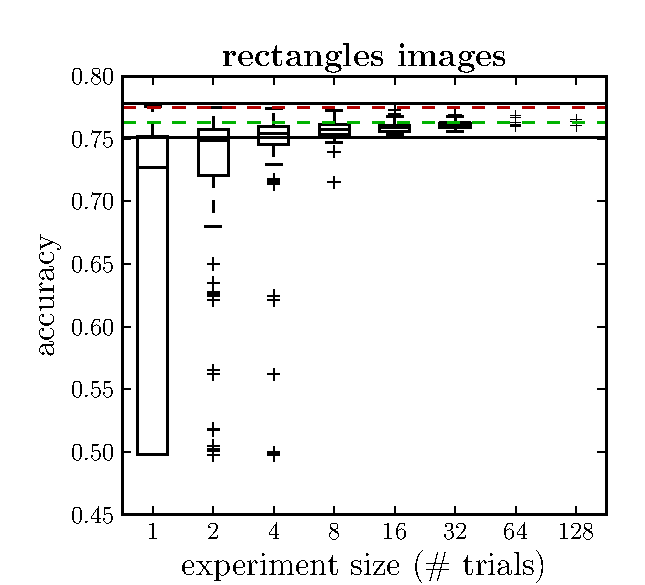
\includegraphics[scale=0.37]{figures/dbn_efficiency/dbn_efficiency_rectangles_images}
\vs{2}
    \caption
    {Deep Belief Network (DBN) performance according to random search.
    Random search is used to explore up to 32 hyper-parameters (see Table~\ref{tbl:dbnprior}).
    Results found using a grid-search-assisted manual search over a similar domain with
    an average 41 trials are given in green (1-layer DBN) and red (3-layer DBN).
    Each box-plot (for $N=1,2,4,...)$ shows the distribution of test set performance when the best model among
    $N$ random trials is selected. The datasets ``convex'' and ``mnist rotated
    background images'' are used for more thorough hyper-parameter
    optimization.
    }
    \label{fig:dbn_random_efficiency}
\end{minipage}
\vs{3}
\end{figure}


\Bs
\section{Sequential Search for Hyper-Parameter Optimization in DBNs}

\label{sec:exp}
%\as
%\subsection{Validating surrogate modelling on the Boston Housing dataset}
%\ass
We validated our GP approach of Section \ref{ss:ea} by comparing
with random sampling on the Boston
Housing dataset, a regression task with 506 points made of 13 scaled
input variables and a scalar regressed output. We trained a
Multi-Layer Perceptron (MLP) with 10 hyper-parameters,
including learning rate, $\ell_1$ and $\ell_2$ penalties, size of hidden
layer, number of iterations, whether a PCA pre-processing was to be
applied, whose energy was the only conditional hyper-parameter~\citep{Bis95}. Our
results are depicted in Figure~\ref{fig:boston}. The first 30 iterations
were made using random sampling, while from the $30^{\mathrm{th}}$ on, we
differentiated the random samples from the GP approach trained on the
updated history. The experiment was repeated 20 times. Although the
number of points is particularly small compared to the dimensionality,
the surrogate modelling approach finds noticeably better points than
random, which supports the application of SMBO approaches to
more ambitious tasks and datasets.

Applying the GP to the problem of optimizing DBN performance,
we allowed 3 random restarts to the CMA+ES algorithm per proposal $x^*$,
and up to 500 iterations of conjugate gradient method in fitting the
length scales of the GP. The squared
exponential kernel \cite{RaWi06} was used for every node. The CMA-ES part of GPs
dealt with boundaries using a penalty method, the binomial sampling
part dealt with it by nature.
The GP algorithm was initialized with 30 randomly sampled points in $\cH$.
After 200 trials, the prediction of a point $x^*$ using this GP took around 150 seconds.

For the TPE-based algorithm, we chose $\gamma=0.15$ and picked the best among 100 candidates drawn from $\ell(x)$
on each iteration as the proposal $x^*$.  After 200 trials, the prediction of
a point $x^*$ using this TPE algorithm
took around 10 seconds.
TPE was allowed to grow past the initial bounds used with for
random sampling in the course of optimization, whereas the GP and random search
were restricted to stay within the initial bounds
throughout the course of optimization.
The TPE algorithm was also initialized with the same 30 randomly sampled points
as were used to seed the GP.

\begin{table}[t]
\vs{2}
\begin{center}
\begin{tabular}{c@{}c}
%\fbox{
\begin{minipage}{0.43\linewidth}
\begin{center}
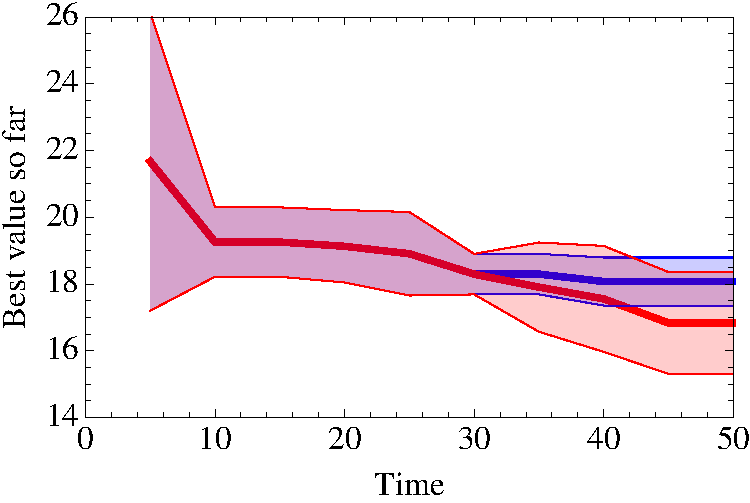
\includegraphics[scale=.39]{figures/bostonHousing.pdf}
\vs{3}
\captionof{figure}{\label{fig:boston}
  After time 30, GP optimizing the MLP hyper-parameters on the Boston
  Housing regression task. Best minimum found so far
  every 5 iterations, against time. Red = GP, Blue = Random. Shaded
  areas = one-sigma error bars.}
\end{center}
\end{minipage}
%}
&
%\fbox{
\hspace*{6mm}\begin{minipage}{0.45\linewidth}
    \begin{center}
    \begin{tabular}{lll}
                & {\bf convex} & {\bf MRBI} \\
        \hline
        TPE & {\bf 14.13} $ \pm 0.30$ \% & {\bf 44.55} $ \pm 0.44$\%   \\
        GP & $ 16.70 \pm 0.32$\% &  $ 47.08\pm 0.44 $\% \\
        Manual & $18.63 \pm 0.34$\%  &  $47.39 \pm 0.44$\%  \\
        Random &  $ 18.97\pm 0.34$ \%  & $50.52 \pm 0.44$\% \\
        \hline
    \end{tabular}
    \end{center}
    \caption{The test set classification error of the best model found by each search algorithm on each problem.
    Each search algorithm was allowed up to 200 trials.
    The manual searches used 82 trials for {\bf convex}
    and 27 trials {\bf MRBI}.
    \label{tbl:testerr}
    }
\end{minipage}
%}
\end{tabular}
\end{center}
\vs{6}
\end{table}


\Bss
\subsection{Parallelizing Sequential Search}
\ass

Both the GP and TPE approaches were actually run asynchronously
in order to make use of multiple compute nodes and to avoid wasting time
waiting for trial evaluations to complete.
For the GP approach, the so-called
{\it constant liar} approach was used: each time a candidate point $x^*$
was proposed, a fake fitness evaluation equal to the mean of the $y$'s
within the training set $\mathcal{D}$ was assigned temporarily, until the
evaluation completed and reported the actual loss $f(x^*)$.
For the TPE approach, we simply ignored recently proposed points and relied
on the stochasticity of draws from $\ell(x)$ to provide
different candidates from one iteration to the next.
The consequence of parallelization is that each proposal $x^*$ is based on
less feedback. This makes search less efficient, though faster in terms of
wall time.

%For the TPE-based algorithm, we choose $\gamma=0.15$ and picked the best among 100 candidates drawn from $\ell(x)$
%on each iteration as the proposal $x^*$.  After 200 trials, the prediction of
%a point $x^*$ using this TPE algorithm
%took around 10 seconds.
%TPE was allowed to grow past the initial bounds used with for
%random sampling in the course of optimization, whereas the GP (and random search)
%was restricted (due simply to implementation details) to stay within the initial bounds
%throughout the course of optimization.
%For comparison, we also evaluated many randomly-chosen trials from the initial 
%sampling distribution (457 and 361 from {\bf convex} and {\bf MRBI} respectively).

Runtime per trial was limited to 1 hour of GPU computation regardless of whether execution was on a GTX 285, 470, 480, or 580. The difference in speed between the slowest and fastest machine was roughly two-fold in theory, but the actual efficiency of computation depended also on the load of the machine and the configuration of the problem (the relative speed of the different cards is different in different hyper-parameter configurations).
With the parallel evaluation of up to five proposals from the GP and TPE algorithms, each experiment took about 24 hours of wall time using five GPUs.


\Bs
\section{Discussion}
\label{sec:discussion}
\as

The trajectories ($\cH$) constructed by each algorithm up to 200 steps are
illustrated in Figure~\ref{fig:H},
and compared with random search and the manual search carried out in
\citet{Larochelle+etal:2007}.
The generalization scores of the best models found using these algorithms and others are listed in Table~\ref{tbl:testerr}.
On the {\bf convex} dataset (2-way classification), both algorithms converged
to a validation score of 13\% error.
In generalization, TPE's best model had 14.1\% error and GP's best had 16.7\%.
TPE's best was significantly better than both manual search (19\%) and random search with 200 trials (17\%).
On the {\bf MRBI} dataset (10-way classification), random search was the worst performer (50\%
error), the GP approach and manual search approximately tied (47\% error), while the
TPE algorithm found a new best result (44\% error).
The models found by the TPE algorithm in particular are better than previously
found ones on both datasets.
The GP and TPE algorithms were slightly less efficient than manual
search: GP and EI identified performance on par with manual search within
80 trials, the manual search of \cite{Larochelle+etal:2007} used 82 trials for
{\bf convex} and 27 trials for {\bf MRBI}.

\begin{figure}
\centering
\begin{minipage}{0.9\linewidth}
% /home/bergstra/cvs/hyperopt/hyperopt/dbn.py plot_histories mongo://localhost:20111/dbn_%s_%s/jobs gp3,gm convex 0 2000
  \vs{0}
    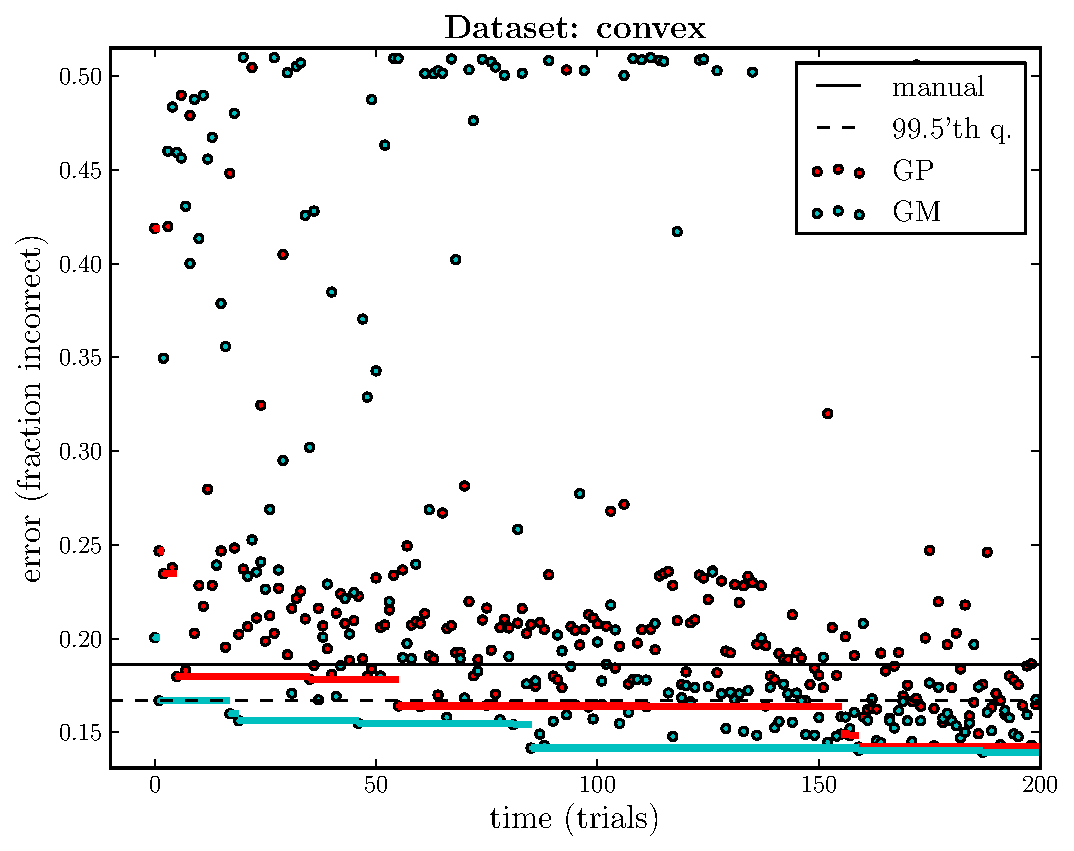
\includegraphics[scale=.35]{figures/plot_histories_gp3,gm_convex.pdf}
    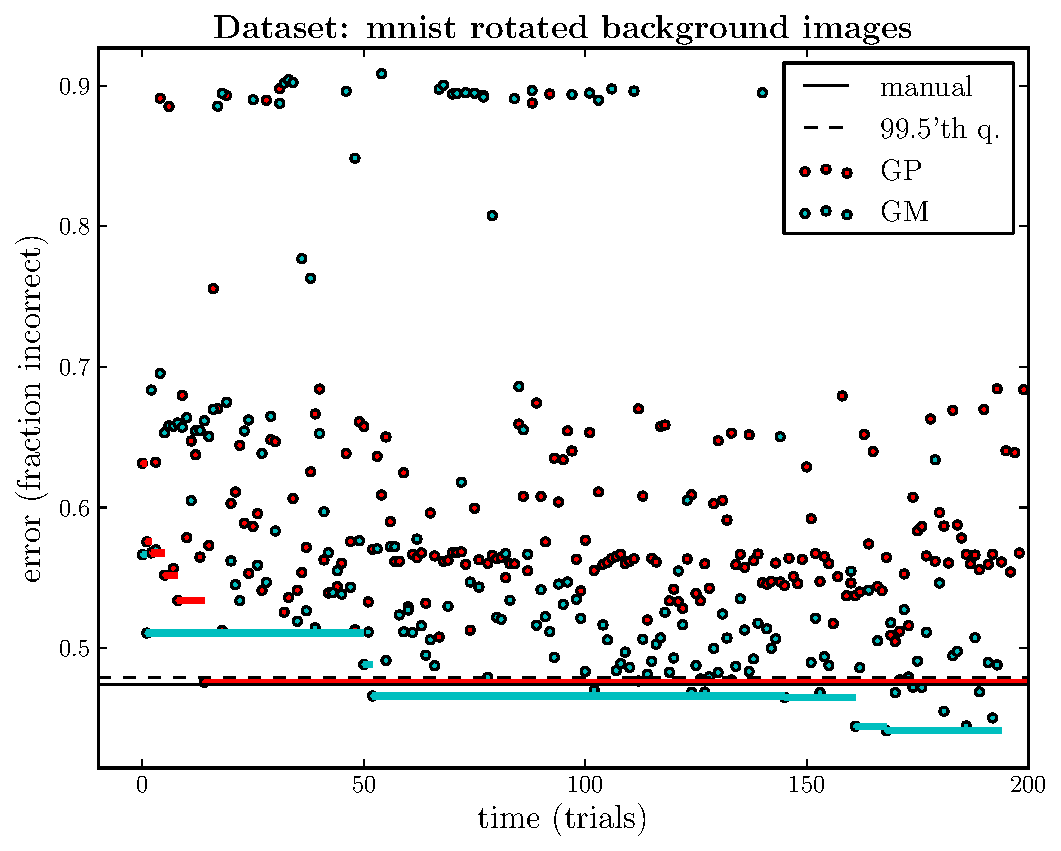
\includegraphics[scale=.35]{figures/plot_histories_gp3,gm_mnist_rotated_background_images.pdf}
  \vs{6}
% /home/bergstra/cvs/hyperopt/hyperopt/dbn.py plot_histories mongo://localhost:20111/dbn_%s_%s/jobs gp3,gm mnist_rotated_backgound_images 0 2000
    \caption{Efficiency of Gaussian Process-based (GP) and graphical
    model-based (TPE) sequential optimization algorithms on the task of optimizing the validation set performance of a DBN of up to three layers on the {\bf convex} task (left) and the {\bf MRBI} task (right).
    The dots are the elements of the trajectory $\cH$ produced by each SMBO algorithm.
    The solid coloured lines are the validation set accuracy of the best trial found before each point in time.
    Both the TPE and GP algorithms make significant advances from their random
    initial conditions, and substantially outperform the manual and random
    search methods. A 95\% confidence interval
    about the best validation means on the {\bf convex} task extends 0.018 above and below each point,
    and on the {\bf MRBI} task extends 0.021 above and below each point.
    The solid black line is the test set accuracy obtained by domain experts using a combination
    of grid search and manual search~\citep{Larochelle+etal:2007}.
    The dashed line is the 99.5\% quantile of validation performance found among trials sampled from our prior distribution (see Table~\ref{tbl:dbnprior}),
    estimated from 457 and 361 random trials on the two datasets respectively.
    % convex has n=1500 validation points
    % best scores have Bernoulli param p = 0.15
    % variance is 1.96 sqrt(p * (1-p)/n) = 0.018%
    % MRBI has n=2000 validation points, p=.45
    }
  \vs{4}
    \label{fig:H}
\end{minipage}
\end{figure}



%Look at some of the scatter plots - which parameters turned out to be most important?

%We added the possibility of ZCA pre-processing, did it help any?

%What about depth - what do the optimization algorithms choose for the number of layers?

%What is a good termination condition for these sequential algorithms?

There are several possible reasons for why the TPE approach outperformed the GP approach in
these two datasets.
Perhaps the inverse factorization of $p(x|y)$ is more accurate than
the $p(y|x)$ in the Gaussian process.
Perhaps, conversely, the exploration induced by the TPE's lack of accuracy
turned out to be a good heuristic for search.
Perhaps the hyper-parameters of the GP approach itself were not set
to correctly trade off exploitation and exploration in the DBN configuration
space.
More empirical work is required to test these hypotheses.
Critically though, all four SMBO runs matched or exceeded both random search
and a careful human-guided search,
which are currently the state of the art methods for hyper-parameter optimization.

%The latter cause might express the need for more ``aggressive'' criteria
%than EI, i.e. switching ``earlier'' than EI to an exploitation mode.  
%The difference in their ordering could be a statistical anomaly
% - let the reviewer point that one out, and hopefully we'll be ready with
%   error bars by the time the review period comes along.

The GP and TPE algorithms work well in both of these settings,
but there are certainly settings in which these algorithms, and in fact SMBO
algorithm in general, would not be expected to do well.
Sequential optimization algorithms work by leveraging structure in observed
$(x,y)$ pairs.
It is possible for SMBO to be arbitrarily bad with a bad choice of $p(y|x)$.
It is also possible to be slower than random sampling at finding a global
optimum with a apparently good $p(y|x)$,
if it extracts structure in $\cH$ that leads only to a local optimum.


%XXX ANALYSIS OF RANDOM SEARCH
%In a follow-up study, \citet{bergstra+bengio:2012accepted} looked at random trials
%showed that random search can be much more
%efficient than grid search in settings where not all hyper-parameters are
%equally relevant.
%for optimizing DBNs as in 
%Random experiments were competitive with the manual sequential optimization of DBNs for
%the majority of data sets,
%even though a grid search would not have been feasible.


\Bs
\section{Conclusion}
\label{sec:conclusion}
\as

This paper has introduced two sequential hyper-parameter optimization algorithms,
and shown them to meet or exceed human performance and the performance of a brute-force random search
in two difficult hyper-parameter optimization tasks involving DBNs.
We have relaxed standard constraints (e.g. equal layer sizes at all layers) on the search space,
and fall back on a more natural hyper-parameter space of 32 variables
(including both discrete and continuous variables)
in which many variables are sometimes irrelevant,
depending on the value of other parameters (e.g. the number of layers).
In this 32-dimensional search problem,
the TPE algorithm presented here has uncovered new best results on both of these datasets that are significantly better than what DBNs were previously believed to achieve.
Moreover, the GP and TPE algorithms are practical: the optimization for each dataset was done in just 24 hours using five GPU processors.
Although our results are only for DBNs, our methods are quite general,
and extend naturally to any hyper-parameter optimization problem in which the hyper-parameters are drawn from a measurable set.

We hope that our work may spur researchers in the machine learning community
to treat the
hyper-parameter optimization strategy as an interesting and important
component of all learning algorithms.
The question of ``How well does a DBN do on the {\bf convex} task?'' is not a
fully specified,
empirically answerable question --
different approaches to hyper-parameter optimization will give different answers.
Algorithmic approaches to hyper-parameter optimization make machine learning results easier to disseminate, reproduce, and transfer to other domains.
The specific algorithms we have presented here are also capable, at least in
some cases, of finding better results than were previously known.
Finally, powerful hyper-parameter optimization algorithms broaden the horizon
of models that can realistically be studied; researchers need not restrict themselves to systems of a few variables that can readily be tuned by hand.

The TPE algorithm presented in this work, as well as parallel evaluation
infrastructure, is available as BSD-licensed free
open-source software, which has been designed not only to reproduce the
results in this work, but also to facilitate the application of these and
similar algorithms to other hyper-parameter optimization problems.\footnote{
``Hyperopt'' software package: \url{https://github.com/jaberg/hyperopt}}

\subsection*{Acknowledgements}
This work was supported by the National Science and Engineering Research
Council of Canada, Compute Canada, and by the ANR-2010-COSI-002 grant of the French National Research Agency.
GPU implementations of the DBN model were provided by
Theano~\cite{bergstra+etal:2010}.


\newpage
\small
\bibliographystyle{unsrt}
\bibliography{strings,strings-short,strings-shorter,jb,hyperoptim}

\end{document}

\iffalse
Vincent+etal:2010 used it. They found the SDA3 model superior to DBN3 on both datasets.
SDA3 model scored $43.76 \pm 0.43$ on {\bf MRBI} and $19.06 \pm 0.34$ on {\bf convex}.
Our findings do not change the ordering of DBN-3 and SDA-3 on these datasets,
but whereas before the SDA was clearly better on {\bf MRBI} and nearly as good on {\bf convex},
our results turn the table: the DBN is clearly better on {\bf convex} and nearly as good on {\bf MRBI}.
\fi


def stack(N):
    return rSON2(
        'learningrate', expon(),
        'l1', expon(),
        'l2', expon(),
        'finetune', TrueFalse())

'conf', rson2(
    'preprocessing', oneof( 'zca', 'lcn'),
)

P(x) = probability that x is worth trying.


On each iteration, we seek an x that maximizes EIR.

\begin{align}
\vs{.5}
EI_{y^*}(x) &= \int_{0}^{y^*} P(y|x) (y^* - y) dy \\
&= \int_{0}^{y^*} P(x|y)P(y)/P(x) (y^* - y) dy \\
&= \frac
{\int_{0}^{y^*} P(x|y)P(y) (y^* - y) dy}
{\int_y' P(x|y')P(y')}
%&= y^* \int_{0}^{y^*} P(y|x) - \int_{0}^{y^*} P(y|x) y dy \\
%&= y^* \int_{0}^{y^*} P(x|y)P(y)/P(x) - \int_{0}^{y^*} P(x|y)P(y)/P(x) y dy \\
\vs{.5}
\end{align}

\Bs
\section{Expected Improvement Rate}
\as

A greedy algorithm for searching good hyper-parameter values optimizes the rate at which our best current model improves.
To evaluate a point $x$ requires CPU time (call this $\mathrm{runtime}(x)$ that returns wall-time in some unit of time).
This suggests a simple extension to the common \emph{expected improvement} search criterion:
maximize expected improvement / CPU time.
\begin{align}
\vs{.5}
    \mathrm{EI}_{y^*}(x) &= \int_{-\infty}^{y^*} \mathrm{P}(y|x) (y^* - y) dy \\
    \mathrm{EIR}_{y^*}(x) &= \frac{\mathrm{EI}_{y^*}(x)}{\mathrm{runtime}(x)}
\vs{.5}
\end{align}
where $y$ is the validation error obtained with hyper-parameters setting $x$.



\subsection{Searching with EIR (YB: IS THIS STILL RELEVANT?)}

A search algorithm based on EIR is the following:

\begin{enumerate}
    \item Initialize $P_0(y,x)$ to prior.
    \item Initialize $\mathrm{runtime_0}()$ to prior.
    \item Initialize experimental data to null set \{\}.
    \item Repeat until stopping condition met:
        \begin{enumerate}
            \item Find a point $x_t$ that maximizes EIR, based on density $P_t$, $\mathrm{runtime}_t$.
            \item Evaluate $x_t$ to get score $y_t$ and measure the time ($r_t$) that it took.
            \item Add $(x_t, y_t, r_t)$ to the set of experimental data.
            \item Revise density $P_t$ and runtime estimator $\mathrm{runtime}_t$ based on this data, obtain $P_{t+1}$, $\mathrm{runtime}_{t+1}$.
        \end{enumerate}
\end{enumerate}


While random search can be surprisingly efficient, it is a brute force method
that suffers from the curse of dimensionality~\citep{bellman:1961}.
Sequential search methods, which use the results of earlier trials to guide
the choice of later ones, are more promising in high-dimensional spaces.
This paper introduces two practical, scalable sequential methods
that improve on random search and grid search in optimization problems where
these methods fall short of human performance (manual optimization).
The algorithms presented here are moderately parallelizable,
in the sense that sequential optimization can be projected a few steps into the future
in order to run future steps in parallel with the current steps.
This can improve speed with respect to wall time by sacrificing overall computational
efficiency.
The methods are tested on the difficult problem of DBN hyper-parameter optimization,
but they are not DBN-specific; they apply to a broad range of configuration problems involving
fixed or variable numbers of parameters that each might be discrete, ordinal, or continuous.

\iffalse
This paper is structured as follows.
Section~\ref{sec:random} summarizes previous work on the use of random sampling for hyper-parameter optimization. This section also introduces the difficult hyper-parameter optimization problems
that will be the object of our studies involving sequential algorithms.
Section~\ref{sec:smbo} describes sequential model-based global optimization in general,
the expected improvement (EI) criterion that we use to guide our algorithms,
as well as the design choices we made to adapt our sequential optimization algorithms to hyper-parameter optimization (specifically, with regards to the handling of conditionally irrelevant variables).
Section~\ref{sec:exp} provides experimental evidence that these sequential algorithms are able to
match or exceed human performance in the difficult cases where random search was too inefficient.
Section~\ref{sec:discussion} provides additional discussion of our algorithms and results,
and the paper concludes with Section~\ref{sec:conclusion}.
\fi


Recall from Section \ref{ss:GPs} that under a GP model on $f$, we have
$$p(y\vert x,\cF_n) = \cN(\widetilde{m}(x),\widetilde{\sigma}(x)^2),$$
where $\tilde\sigma(x) = \tilde{k}(x,x)^{1/2}$. A direct computation then yields
\begin{equation}\label{e:EIunderGP}
\vs{.5}
 \text{EI}_{y^*}(x)=\widetilde{\sigma}(x)\big(u(x)\Phi(u(x))+\phi(u(x))\big),
\vs{.5}
\end{equation}
where $u(x)=(y^*-\widetilde{m}(x))/\widetilde{\sigma}(x)$, and $\Phi$ and
$\phi$ denote the cdf and pdf of the $\mathcal{N}(0,1)$ distribution,
respectively. This alternative definition makes it easier to remark that EI
encapsulates a compromise between regions where the mean function is
close to or better than the best value obtained so far and
under-explored regions
where the uncertainty is high. The next two subsections describe two different
algorithms that use the EI criterion to propose candidates in step
\ref{ai:candidate} of SMBO.

%been evaluated at $n$ points from $\mathcal{D}:=\{(x_i,f(x_i)) ; 1\leq
%i\leq n\}.$ Assume you
%$\mathcal{F}_n$ is the $\sigma$-algebra generated by the previous
%fitness evaluations summarized in $\mathcal{D}$.
The EI strategy
defines the next point $x_{n+1}$ to be
evaluated as the point where the expected improvement over 
%the currently best minimum $m_n:=\min_i f(x_i)$ 
a user-defined value $y^*\in\mathbb{R}$ is the highest.

